\subsection{Schema Indexing}

To choose the most relevant subset of samples from $\mathcal{S}$ for $k$-shot learning,
it is important that the SQL queries we supply are written for structurally similar SQL schemas
in order to minimize the structural difference between the supplied samples $\mathcal{S}_k$ and
the ground truth query $\omega_{ground}$ for a given natural language question.

For example $\omega_{ground}$ the question ``Give me all contacts for the user with the id 10''
might look different depending on the database schema at hand, thus only selecting
samples based on the similarity of the natural language question will yield inferior
sample quality.

\begin{figure}[ht]
  \vspace{1em}
  \hfill
  \begin{minipage}[b]{0.45\linewidth}
    \begin{verbatim}
CREATE TABLE users (
  id TEXT PRIMARY KEY
);

CREATE TABLE contacts (
  user_id TEXT NOT NULL,
  name TEXT NOT NULL,
  FOREIGN KEY (user_id) ON users(id),
  PRIMARY KEY (user_id, name)
);
    \end{verbatim}
    \caption{Normalized schema}
    \label{figure:schema-normalized}
  \end{minipage}
  \hfill
  \begin{minipage}[b]{0.35\linewidth}
    \begin{verbatim}
CREATE TABLE users (
  id TEXT PRIMARY KEY,
  contacts TEXT[] NOT NULL
);
    \end{verbatim}
    \vspace{3.75em}
    \caption{Denormalized schema}
    \label{figure:schema-denormalized}
  \end{minipage}
  \hfill
  \vspace{1em}
\end{figure}

Given the database schemas in figures~\ref{figure:schema-normalized} and~\ref{figure:schema-denormalized}
respective definitions of $\omega_{ground}$ would be:

\begin{figure}[ht]
  \vspace{1em}
  \hfill
  \begin{minipage}[b]{0.45\linewidth}
    \begin{verbatim}
SELECT contacts.name
FROM users
JOIN contacts
  ON contacts.user_id = users.id
WHERE users.id = 10;
    \end{verbatim}
    \caption{SQL JOIN selection}
    \label{figure:sql-join-example}
  \end{minipage}
  \hfill
  \begin{minipage}[b]{0.35\linewidth}
    \centering
    \begin{verbatim}
SELECT contacts
FROM users
WHERE id = 10;
    \end{verbatim}
    \vspace{1.3em}
    \caption{SQL Array selection}
    \label{figure:sql-array-example}
  \end{minipage}
  \hfill
  \vspace{1em}
\end{figure}


As shown in the figures~\ref{figure:sql-join-example} and~\ref{figure:sql-array-example}
the structural similarity of the underlying database schema is a crucial component
of the relevance of a example.

\subsubsection{Graph Representation}

To determine structural similarity of database schemas, we propose using
graph representation of database schemas as a data definition language (DDL)
independent representation of the database structure. Choosing a graph
representation allows us to leverage established methods for measuring graph similarity
such as Wasserstein-Weisfeiler-Lehman graph kernels \cite{WWL}. % TODO: Add proper WWL citation

Given a database schema $s$, the corresponding graph $G_s = (V, E, \ell, w)$ is defined as:

\begin{enumerate}
    \item $V = V_t \cup V_c$ where $V_t$ represents table nodes and $V_c$ represents column nodes
    \item $E = E_{tc} \cup E_{fk} \cup E_{ref}$ where:
        \begin{itemize}
            \item $E_{tc}$ are table-column edges
            \item $E_{fk}$ are foreign key relationship edges between tables
            \item $E_{ref}$ are reference edges between foreign key columns
        \end{itemize}
    \item Each node $v \in V$ has a semantic label $\ell(v) \in \{1, 2, \ldots, 9\}$ where:
        \begin{itemize}
            \item $\ell(v) = 1$ for table nodes
            \item $\ell(v) = 2$ for generic column nodes
            \item $\ell(v) = 3$ for primary key columns
            \item $\ell(v) = 4$ for foreign key columns
            \item $\ell(v) = 5$ for text columns
            \item $\ell(v) = 6$ for numeric columns
            \item $\ell(v) = 7$ for datetime columns
            \item $\ell(v) = 8$ for boolean columns
            \item $\ell(v) = 9$ for other/unknown data types
        \end{itemize}
    \item Each edge $e \in E$ has a weight $w(e) \in \{0.5, 0.9, 1.0\}$ reflecting structural importance:
        \begin{itemize}
            \item $w(e) = 1.0$ for foreign key relationships (highest importance)
            \item $w(e) = 0.9$ for column reference edges
            \item $w(e) = 0.5$ for table-column edges
        \end{itemize}
\end{enumerate}

We define the structural similarity of two databases as the topological distance
of the respective graphs. The graph representation captures essential schema
structure through semantic node labeling that prioritizes constraints over data
types: primary key columns receive label 3 regardless of their underlying data
type, foreign key columns receive label 4, and only then are remaining columns
categorized by data type (text=5, numeric=6, datetime=7, boolean=8, other=9).
This hierarchical labeling ensures that structural relationships take
precedence over semantic content, while omitting table names, column names and
domain terminology to achieve schema-agnostic comparison.

The graph representation of the database schemas described in~\ref{figure:schema-normalized}
and~\ref{figure:schema-denormalized} are therefore:

\begin{figure}[ht]
  \vspace{1em}
  \hfill
  \begin{minipage}[b]{0.45\linewidth}
    \centering
    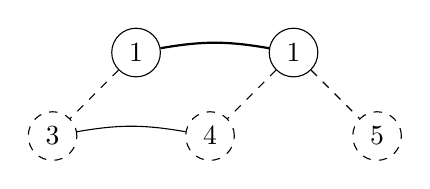
\begin{tikzpicture}[node distance={15mm}, table/.style = {draw,circle}, column/.style = {draw,dashed,circle}]

      \node[table] (users) at (0,0) {1}; 
      \node[table] (contacts) at (2,0) {1}; 
      
      \node[column] (users_id) [below left of=users] {3}; 
      
      \node[column] (contacts_user_id) [below left of=contacts] {4};
      \node[column] (contacts_name) [below right of=contacts] {5};
      
      \draw[dashed] (users) -- (users_id); 
      \draw[dashed] (contacts) -- (contacts_user_id); 
      \draw[dashed] (contacts) -- (contacts_name); 
      
      \draw[thick] (users) to [out=10, in=170] (contacts);
      
      \draw (users_id) to [out=10, in=170] (contacts_user_id); 
    \end{tikzpicture} 
    \caption{Normalized graph repr.}
    \label{figure:normalized-graph-representation}
  \end{minipage}
  \hfill
  \begin{minipage}[b]{0.45\linewidth}
    \centering
    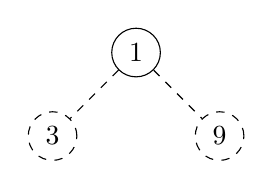
\begin{tikzpicture}[node distance={15mm}, table/.style = {draw,circle}, column/.style = {draw,dashed,circle}]
      \node[table] (users) at (0,0) {1}; 
      
      \node[column] (users_id) [below left of=users] {3}; 
      \node[column] (users_contacts) [below right of=users] {9};
      
      \draw[dashed] (users) -- (users_id); 
      \draw[dashed] (users) -- (users_contacts); 
    \end{tikzpicture} 
    \caption{Denormalized graph repr.}
    \label{figure:denormalized-graph-representation}
  \end{minipage}
  \hfill
  \vspace{1em}
  
  \begin{minipage}{\linewidth}
    \centering
    \vspace{0.5em}
    \small
    \textbf{Legend:} Solid circle = table (1), dashed circle = column (3,4,5), 
    thick line = fk relationship ($w$=1.0), line = reference ($w$=0.9), 
    dashed line = table-column ($w$=0.5)
  \end{minipage}
\end{figure}

The $\delta$ of the order of the graphs~\ref{figure:normalized-graph-representation}
and~\ref{figure:denormalized-graph-representation}
further highlight the structural difference between the two schemas.

\subsubsection{Distance Measurement}

To measure the distance between the graphs displayed in~\ref{figure:normalized-graph-representation}
and~\ref{figure:denormalized-graph-representation}, we employ the
Wasserstein-Weisfeiler-Lehman (WWL) graph kernel method \cite{WWL}. % TODO: Fix WWL citation

The WWL kernel computes structural similarity by combining discrete Weisfeiler-Lehman
graph features with continuous optimal transport theory. The method first extracts
WL features from the labeled graph structure, then computes the Wasserstein distance
between the resulting feature distributions. For two \textsc{Natural}-graphs $G_1$ and $G_2$
with semantic node labels, the distance is computed as:

\begin{equation}
% TODO: Add missing WWL distance formula 
%d_{WWL}(G_1, G_2) = W_2(\mu_{G_1}, \mu_{G_2})
\end{equation}

where $W_2$ denotes the 2-Wasserstein distance and $\mu_{G_i}$ represents the empirical
measure over WL features extracted from graph $G_i$. The semantic node labels
$\ell(v) \in \{1, \ldots, 9\}$ guide the feature extraction process, ensuring that
structurally and semantically similar schema elements contribute similarly to the
distance calculation.

For the example schemas above, the normalized schema (5 nodes, 7 edges) and
denormalized schema (3 nodes, 2 edges) exhibit significant topological differences.
The WWL distance captures both the reduction in graph complexity (fewer nodes and edges)
and the loss of relational structure (elimination of foreign key relationships),
resulting in a substantial distance value reflecting their structural dissimilarity
despite representing equivalent logical relationships.

% TODO: Complete distance calculation example with actual values
% TODO: Add discussion of how semantic labeling affects distance calculation  
% TODO: Clarify relationship between edge weights and WWL computation
% TODO: Add example showing how label priority affects similarity scores

The schema distance index $\mathcal{D}$ maintains precomputed distances between
all observed database schemas, enabling efficient retrieval of structurally similar
databases during sample selection. This index is constructed as a set of
schema-distance tuples $\{(s_1, d_1), \ldots, (s_i, d_i)\}$ where $s_i$ represents
a database schema and $d_i$ denotes its topological distance to the current target
schema. The computational complexity of WL kernel calculation is $O(h \cdot |E|)$
where $h$ is the number of iterations and $|E|$ is the number of edges, making
it practical for real-time schema comparison in moderately sized databases.

% TODO: Fix inconsistent notation: use consistent variable names (G_s vs Natural-graphs)
% TODO: Improve transition between graph definition and distance measurement sections
